\section{Translational Controllers} \label{sec:TranslationalController}

The translational controllers handle the movement of the quadcopter along the inertial frame directions, $x_{\mathrm{I}}$, $y_{\mathrm{I}}$ and $z_{\mathrm{I}}$. The overall diagram in \autoref{fig:ControlHeadDiagram} is rearranged to illustrate the translational controller design structure in \autoref{fig:TranslationalControlDiagram}.
%
\begin{figure}[H]
	\centering
	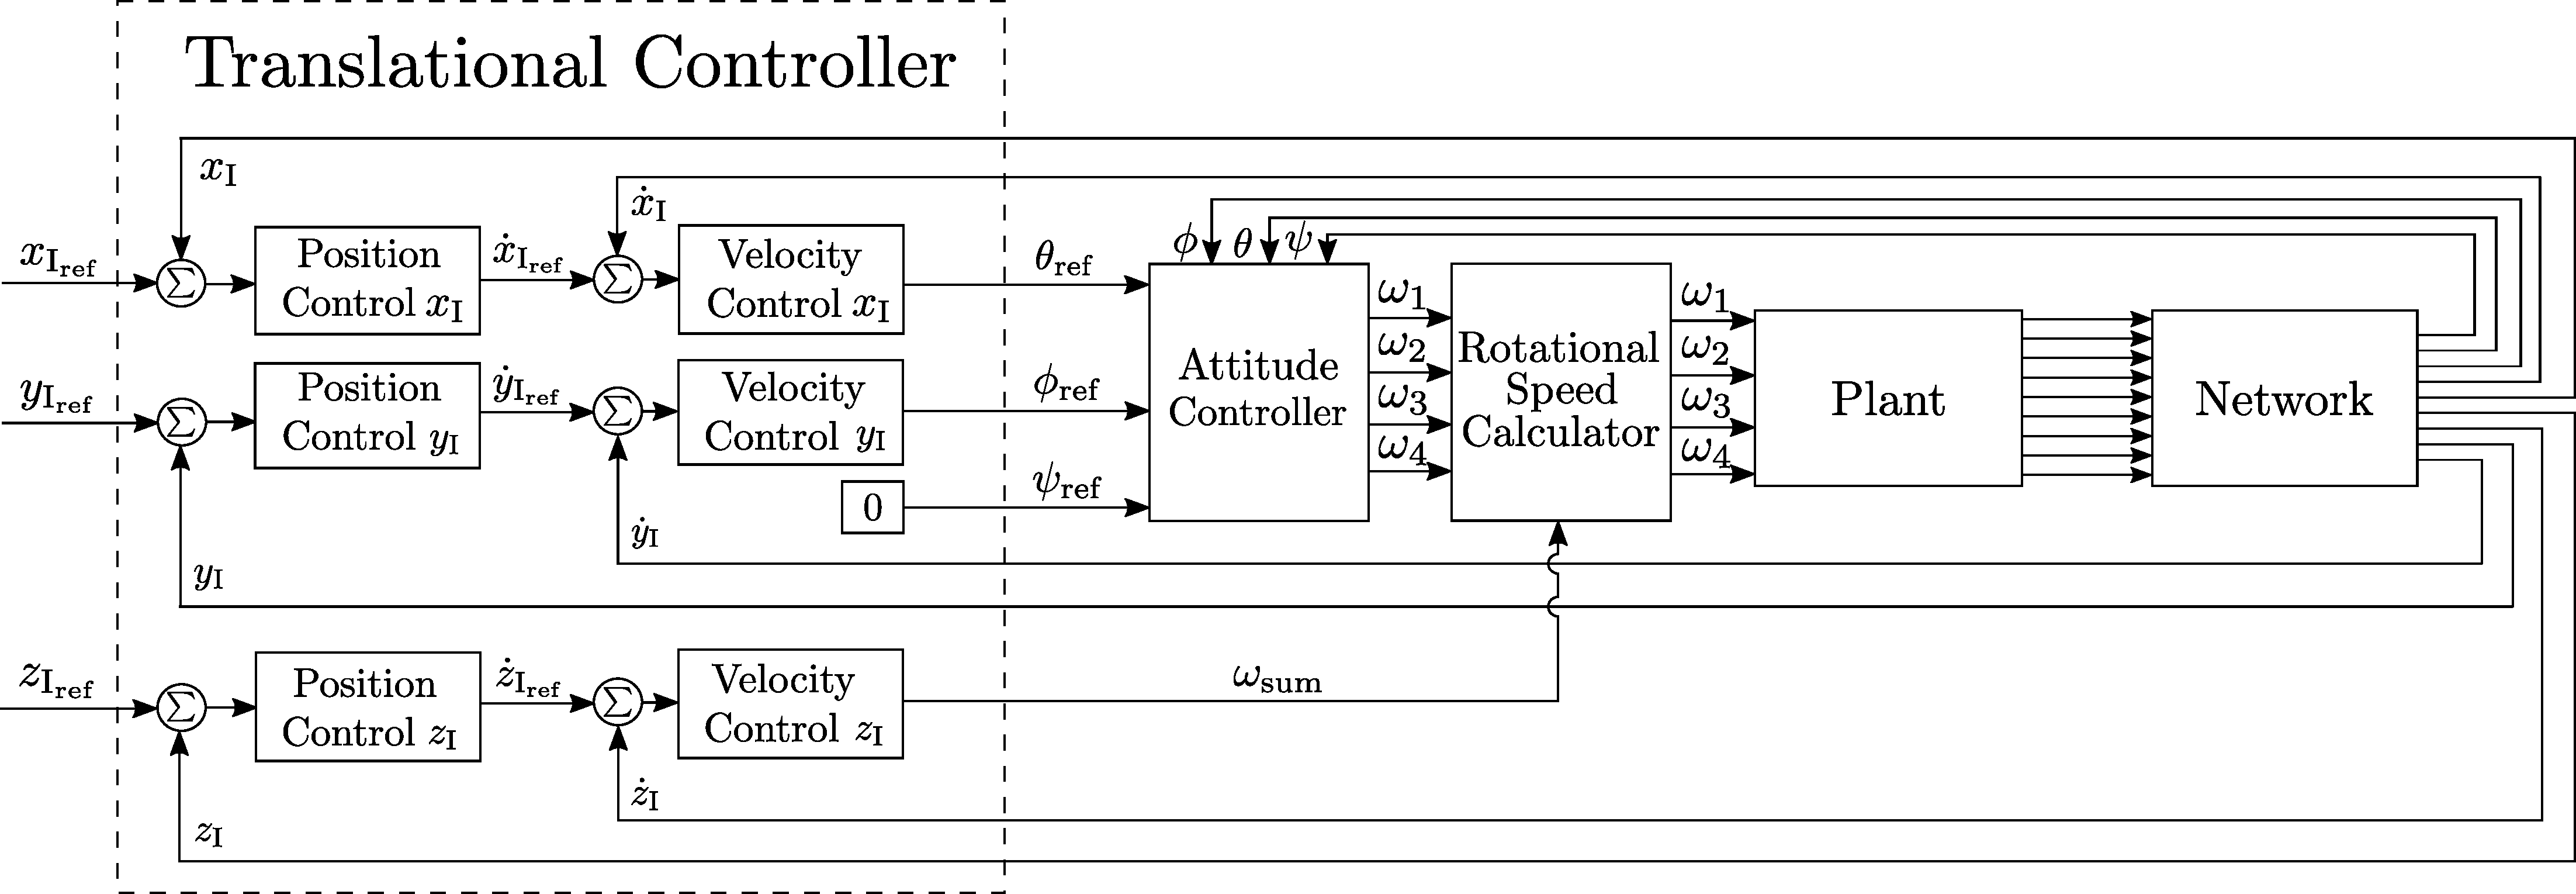
\includegraphics[scale=0.22]{figures/TranslationalControlDiagramexpanded}
	\caption{The overall translational control design structure.}
	\label{fig:TranslationalControlDiagram}
\end{figure}
%
For each axis, the velocity and position controllers form a cascade control structure, where the position controller sets the reference for the velocity controller. In the figure, it is also possible to see how $x_{\mathrm{I}}$ and $y_{\mathrm{I}}$ controllers share similar properties as both have as output an angle reference for the attitude controller, $\theta_{\mathrm{ref}}$ and $\phi_{\mathrm{ref}}$, respectively. 
The $z_{\mathrm{I}}$ velocity controller sets the required sum of motor rotational speeds, $\omega_{\mathrm{sum}}$, such that the vertical position is attained.

In the following sections the design for the mentioned controllers is explained.